\documentclass{standalone}
\usepackage{pgfplots}
\pgfplotsset{
  compat=1.18, 
  ticklabel style = {font=\footnotesize},
  axis equal image,
}

\begin{document}
  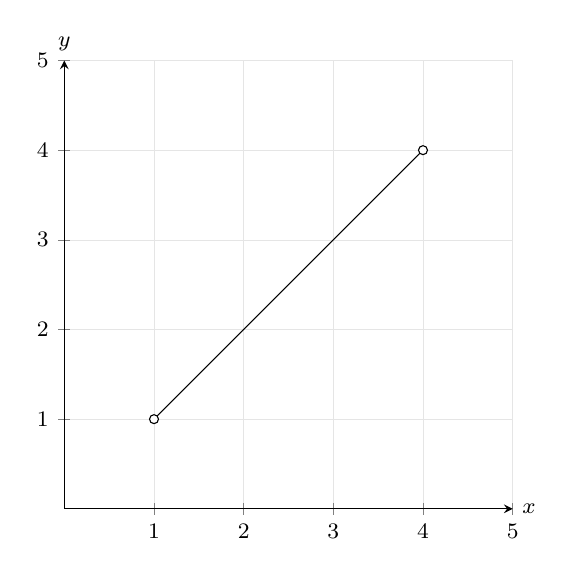
\begin{tikzpicture}
    \begin{axis}[
      axis lines=middle,
      % width=5in, height=5in,
      xmin=0, xmax=5,
      ymin=0, ymax=5,
      xlabel={\footnotesize \(x\)},
      xlabel style={at={(ticklabel* cs:1)}, anchor=west},
      ylabel={\footnotesize \(y\)},
      ylabel style={at={(ticklabel* cs:1)}, anchor=south},
      axis line style = {thin},
      grid=both,
      grid style={line width=.2pt, draw=gray!20},
      % minor tick num=1, 
      ]
      \addplot[no marks] coordinates { (1,1) (4,4) };
      \draw[fill=white] (axis cs:1,1) circle[radius=0.05];
      \draw[fill=white] (axis cs:4,4) circle[radius=0.05];
    \end{axis}
  \end{tikzpicture}
\end{document}

